\chapter{Pénzügyi és statisztikai függvények}
\thispagestyle{empty}

\section{Pénzügyi függvények}

Ebben a kategóriában több mint ötven függvényt találunk,
ezek közül csak néhányat tekintünk át. Az OpenOffice.org
Calc súgójában részletes magyarázatot olvashatunk minden
pénzügyi függvényről.

A \textbf{JBÉ} függvény egy befektetés jövőbeli
értékét adja meg, állandó összegű
befizetések és kamatláb mellett.

Szintaxisa: JBÉ(kamatláb;időszakok\_száma;részlet;jelenérték;típus).
Az első három paraméter kötelező, a két utolsó opcionális.

\Aref{FVFüggvény} ábrán látjuk, hogy elhelyezve százezer forintot
(jelenérték) egy 12\% (kamatláb) évi kamatozású számlán,
és minden hó végén befizetve 20~000 forintot (részlet) 5
éven át (időszakok\_száma), a számlán az öt év
elteltével a JBÉ függvénnyel meghatározható az összeg. 

\begin{figure}[!h]
\begin{center}
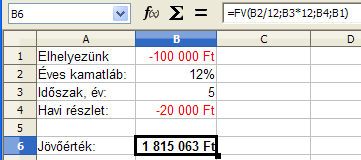
\includegraphics[width=9.55cm]{oocalcv2-img125.png}
\caption{JBÉ függvény}\label{FVFüggvény}
\end{center}
\end{figure}

Figyeljük meg, hogy azok a pénzösszegek, amelyek általunk
befizetésre kerülnek, negatív értékkel szerepelnek, a
hozzánk befolyó összegek pozitív értéket kapnak. A havi
kamatot az éves 12-ed részével adjuk meg (B2/12) és az
időszakok száma szintén hónapokban szerepel (B3*12). A
típus paramétert nem adtuk meg, mert a befizetések a hónapok
végén történnek. Hó eleji törlesztés esetén az
értéke 1 lenne.

Az \textbf{MÉ} (mai érték) függvény segítségével kiszámítható az az
összeg, amelyre --  a mai napon, fix kamatozással befektetve, egy
meghatározott számú időszak múlva --  egy adott összeget
(annuitást) kapunk kézhez.  Megadható, hogy mennyi pénz
maradjon az időszak letelte után. A függvényt a
jelenérték meghatározásának is nevezik.

Szintaxisa: MÉ(kamatláb; időszakok\_száma; részlet;
jövőérték; típus). A jövőérték opcionális
paraméterrel megadhatunk egy elérni kívánt értéket.
Elhagyása esetén 0.

A \textbf{RÉSZLET} függvénnyel egy kölcsönre vonatkozó
törlesztési összeget számíthatunk ki, állandó
összegű törlesztőrészletek és kamatláb esetén.

Szintaxisa:
RÉSZLET(kamatláb;időszakok\_száma;jelenérték;jövőérték;típus).
A jelenérték az a jelenbeli egyösszegű kifizetés, amely
egyenértékű a jövőbeli kifizetések összegével. A
jövőérték opcionális paraméter, az utolsó részlet
kifizetése után elérni kívánt összeg. Amennyiben elhagyjuk,
a függvény 0-nak tekinti.

\Aref{29-feladatPMT} ábrán egy 5 millió forintos, 17\%-os éves
kamatrátájú, 10 év alatt havi részletekben visszafizetendő
kölcsön havi részleteit látjuk.

\begin{figure}[!h]
\begin{center}
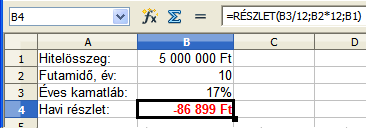
\includegraphics[width=8.206cm]{oocalcv2-img127.png}
\caption{RÉSZLET függvény}\label{29-feladatPMT}
\end{center}
\end{figure}

A kiszámított összeg a tőketörlesztés összegét és a
kamatokat adja meg, a kölcsönhöz kapcsolódó egyéb
költségeket, mint pl. adó vagy kezelési költség nem
tartalmazza. Megszorozva a kiszámított összeget a kifizetések
számával megkapjuk a teljes kifizetendő összeget.
Esetünkben:  10~427~869~Ft.

A \textbf{PRÉSZLET} függvény egy hiteltörlesztésen belül a
tőketörlesztés nagyságát számítja ki egy adott
időszakra, adott nagyságú állandó
törlesztőrészletek és állandó kamatláb mellett.
Szintaxisa: PRÉSZLET(kamat; időszak; időszakok\_száma;
jelenérték; jövőérték; típus). A két utolsó
paraméter opcionális.  A \textbf{jelenérték} az a jelenbéli
egyösszegű kifizetés, amely egyenértékű a
jövőbeli kifizetések összegével. A jövőérték az
utolsó részlet kifizetése után elérni kívánt összeg.
Elhagyása esetén a függvény 0-nak tekinti.

Az \textbf{RRÉSZLET} függvény egy hiteltörlesztésen belül a
kamattörlesztés nagyságát számítja ki egy adott
időszakra, adott nagyságú állandó
törlesztőrészletek és állandó kamatláb mellett.
Paraméterei megegyeznek a PRÉSZLET függvényével.

\Aref{29-feladatPPMT} ábrán egy 6 hónap futamidejű, 200~000~Ft-os hitel
tőke- és kamattörlesztés havi értékeit és azok összegét látjuk.

\begin{figure}[!h]
\begin{center}
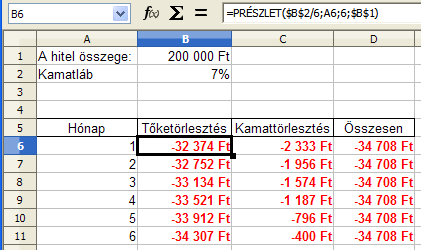
\includegraphics[width=11.137cm]{oocalcv2-img128.png}
\caption{PRÉSZLET függvény}\label{29-feladatPPMT}
\end{center}
\end{figure}

\section{29. feladat}

{\itshape
Vizsgáljuk meg, hogy érdemes-e megvenni 400~000~Ft-ért egy
értékpapírt, ami havi rendszeres 8000~Ft jövedelmet kínál 5
éven át. Az évi kamatláb 14\%.}

Akkor érdemes megvenni az értékpapírt, ha kiszámított
jelenérték 400~000~Ft vagy több. Számítsuk ki az MÉ
függvénnyel (\ref{29-feladatPV} ábra).

\begin{figure}[!h]
\begin{center}
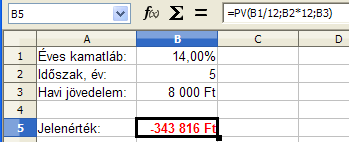
\includegraphics[width=8.232cm]{oocalcv2-img126.png}
\caption{29.  feladat --  MÉ függvény}\label{29-feladatPV}
\end{center}
\end{figure}

Az öt éven át történő kifizetés jelenértéke csak
343~816~Ft, tehát nem érdemes megvenni az értékpapírt.


\section{Statisztikai függvények}

A statisztikai függvények közül az egyszerűbbeket
áttekintettük a negyedik fejezetben. Most vizsgáljunk meg
néhány olyan függvényt ebből a kategóriából,
amelyeket gyakran használnak mind gazdasági elemzéseknél, mind
mérnöki kutatómunka során.

A \textbf{SZÓRÁS} függvény minta alapján becslést ad a
szórásra. A szórás azt méri, hogy az értékek a
várható értéktől (középértéktől) milyen
mértékben térnek el. Szintaxisa: SZÓRÁS(szám1;szám2;...). Az
argumentumok numerikus értékek vagy tartományok. A SZÓRÁS
függvény az argumentumokat statisztikai sokaság mintájának
tekinti. Amikor az adatok a teljes sokaságot jelentik, akkor a
szórást a \textbf{SZÓRÁSP} függvénnyel számítjuk ki. 

A SZÓRÁS függvény a szöveges és a logikai értékeket
figyelmen kívül hagyja. A \textbf{SZÓRÁSA} függvény a
szórást úgy számítja ki, hogy a szöveget és a HAMIS
logikai értéket nullának, az IGAZ logikai értéket pedig 1-nek
tekinti. A teljes sokaságra vett szórást, a logikai és
szöveges argumentumokat is figyelembe véve a \textbf{SZÓRÁSPA}
függvénnyel számítjuk ki.

A \textbf{MEDIÁN} függvény kiszámítja a számhalmaz
középső értékét. Páratlan számú értéket
tartalmazó halmazban a középső érték a halmaz közepén
elhelyezkedő érték. Páros számú értéket tartalmazó
halmazban a középső érték a halmaz közepén
elhelyezkedő két érték átlaga. Szintaxisa:
MEDIÁN(szám1;szám2;...). A szöveget, a logikai értékeket és
üres cellákat figyelmen kívül hagyja.

A \textbf{MÓDUSZ} függvény kiszámítja az adathalmazban
leggyakrabban előforduló értéket. Amikor több, egyező
gyakorisággal rendelkező érték létezik, akkor a
függvény eredményül a legkisebbet adja. Hibát ír ki, ha egy
érték nem jelenik meg legalább kétszer. A szöveget, logikai
értékeket és üres cellákat figyelmen kívül hagyja.

A \textbf{MÉRTANI.KÖZÉP} függvény kiszámítja egy minta mértani
közepét. Az argumentumai számok, számokat tartalmazó
tömbök, nevek, vagy hivatkozások lehetnek. Negatív számokat
és nullát nem tartalmazhat az argumentum. A szöveget, logikai
értékeket és üres cellákat figyelmen kívül hagyja. Két
szám esetén a mértani közép a két szám szorzatának a
négyzetgyökével egyenlő.

\Aref{StatisztikaiFüggvények2}  ábrán a tárgyalt statisztikai függvények
eredményeit látjuk az A2:A11 tartományba írt számhalmazra.

\begin{figure}[!h]
\begin{center}
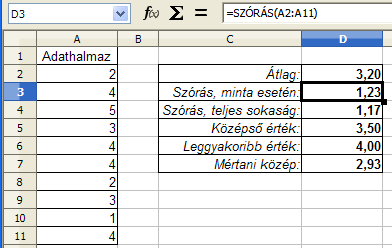
\includegraphics[width=10.37cm]{oocalcv2-img129.png}
\caption{Statisztikai függvények}\label{StatisztikaiFüggvények2}
\end{center}
\end{figure}

Az ebben a fejezetben tárgyalt függvények \aref{15-fejezetFüggvények}
táblázatban láthatóak.

\begin{table}[!h]
\begin{center}
\caption{A fejezetben tárgyalt függvények}\label{15-fejezetFüggvények}
\begin{tabular}{|m{3cm}|m{8cm}|m{3.5cm}|}
\hline
\multicolumn{1}{|c|}{\textbf{A függvény}}&
\multicolumn{1}{c|}{\textbf{Funkciója}}&
\multicolumn{1}{c|}{\textbf{A függvény}} \\
\multicolumn{1}{|c|}{\textbf{neve}} & &
\multicolumn{1}{c|}{\textbf{angol neve}} \\
\hline
JBÉ & Egy befektetés jövőbeli értékét számítja ki. & FV\\ \hline
MÉ & Egy befektetés mai értékét számítja ki. & PV\\ \hline
RÉSZLET & A kölcsönre vonatkozó törlesztési összeget számítja ki. &
PMT\\ \hline
RRÉSZLET & A kamattörlesztés nagyságát számítja ki. & IPMT\\ \hline
PRÉSZLET & A tőketörlesztés nagyságát számítja ki. & PPMT\\ \hline
SZÓRÁS & Minta alapján becslést ad a szórásra. & STDEV\\ \hline
SZÓRÁSP & Sokaság egészéből kiszámítja annak szórását. & STDEVP\\ \hline
SZÓRÁSA & Minta alapján becslést ad a szórásra. Szöveges és logikai
értékek is lehetnek argumentumok. & STDEVA\\ \hline
SZÓRÁSPA & Sokaság egészéből kiszámítja annak szórását.
Szöveges és logikai értékek is lehetnek argumentumok. & STDEVPA\\ \hline
MEDIÁN & Kiszámítja a számhalmaz középső értékét. & MEDIAN\\ \hline
MÓDUSZ & Kiszámítja az adathalmazban leggyakrabban előforduló
értéket. & MODE\\ \hline
MÉRTANI.KÖZÉP & Kiszámítja egy minta mértani közepét. & GEOMEAN\\ \hline
\end{tabular}
\end{center}
\end{table}

